\begin{figure}[t]
  \centering
  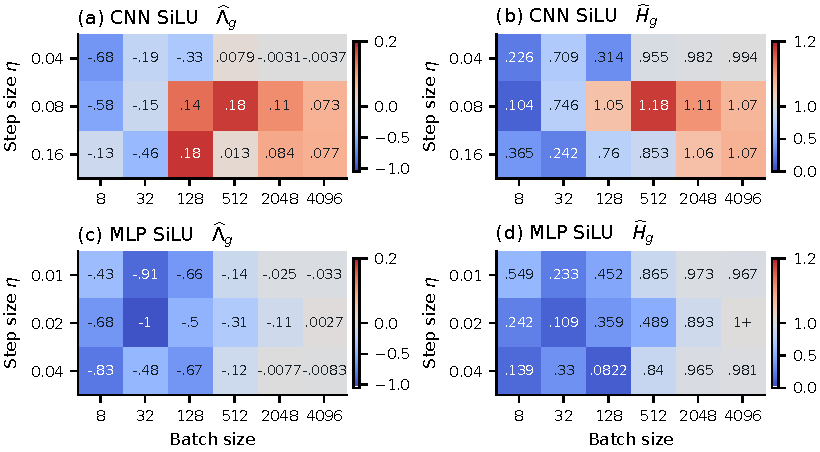
\includegraphics[width=\linewidth]{figures/empirical_stability_heatmaps.pdf}
  \caption{\textbf{Neural networks show distinct scalar diagnostic regimes.}
  Plain SGD on 8,192 CIFAR-10 examples with squared loss.
  For each run, the last three available conditional probe sets are pooled to estimate
  $\widehat\Lambda_g=\operatorname{mean}\log|a_g|$ and
  $\widehat H_g=(\operatorname{mean}|a_g|^{-1})^{-1}$; cells average these run-level statistics.
  Color centers are $0$ and $1$; axes use the actual training step size and batch size.
  CNN settings include $\widehat\Lambda_g>0$ on both sides of $\widehat H_g=1$.
  These are checkpoint-window diagnostics, with varying horizons, not equilibrium or full-network stability certificates.
  A trailing $+$ preserves a value just above the displayed reference after rounding.}
  \label{fig:neural-grids}
\end{figure}

\begin{figure}[t]
  \centering
  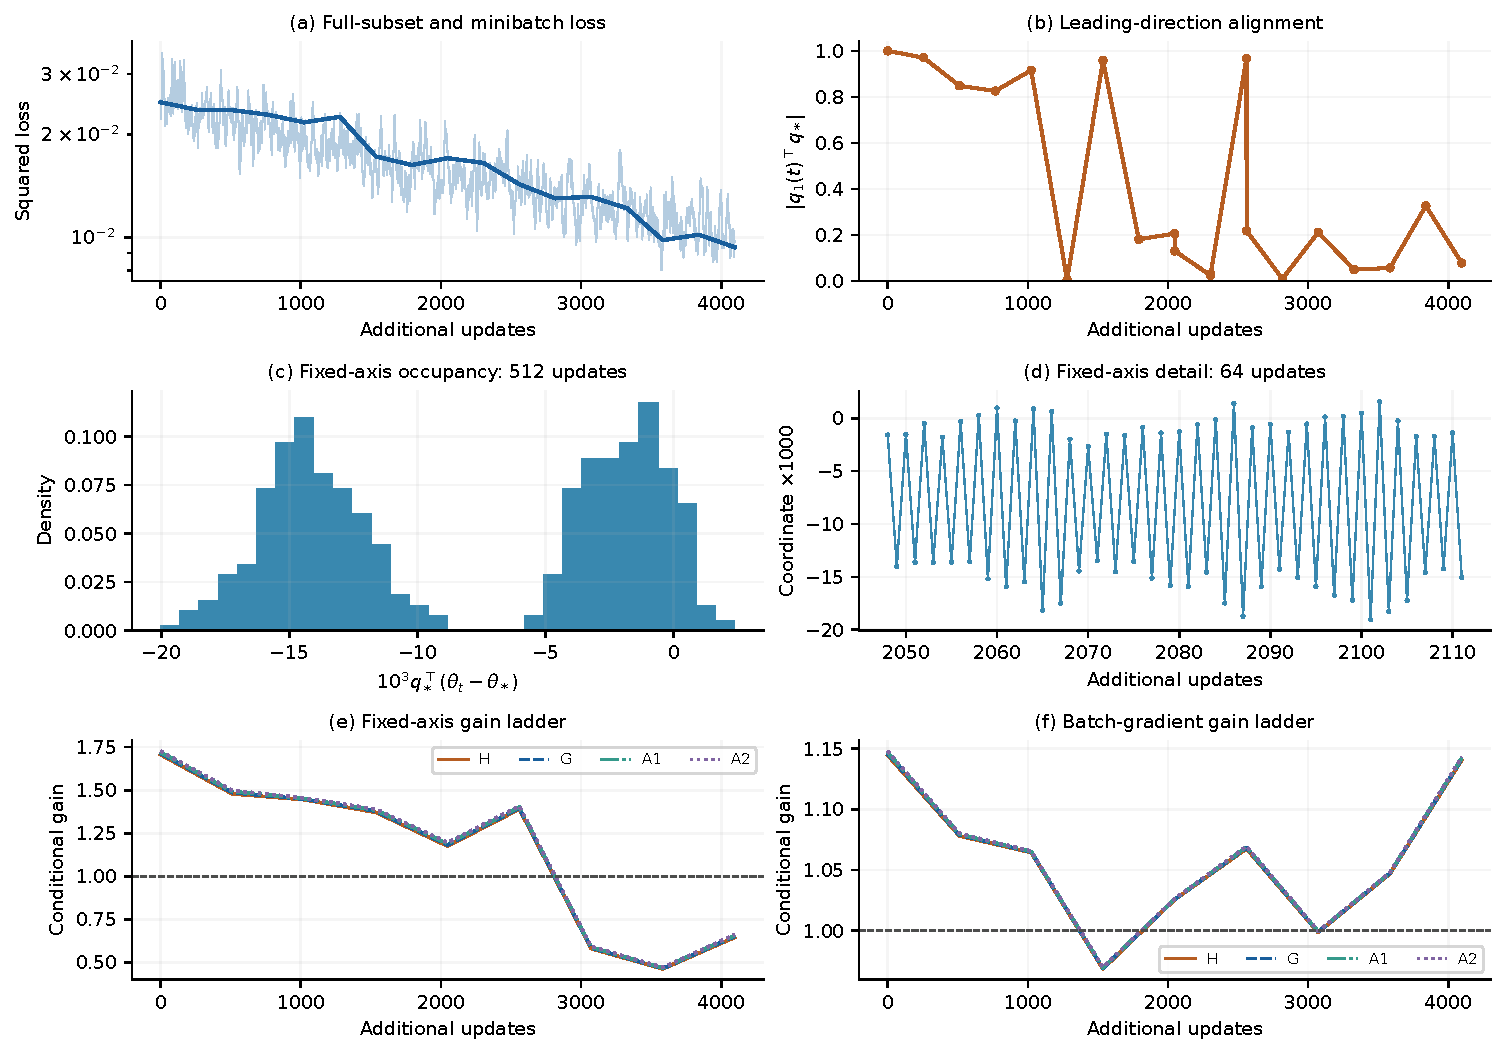
\includegraphics[width=\linewidth]{figures/empirical_iid_mlp_dynamics.pdf}
  \caption{\textbf{Local expansion, two-lobed occupancy, and changing phase coexist.}
  SiLU MLP, CIFAR-10, $B=4096$, $\eta=0.04$, with independently sampled minibatches.
  The reference checkpoint $\theta_\star$ and its leading Hessian Ritz direction $q_\star$ are fixed.
  (a,b) A 64-update trace and its enclosing 512-update occupancy window show alternating lobes across four KDE bandwidths.
  (c) Continuously transported tangent vectors have late growth $+0.00642$ per update; loss decreases from $0.02485$ to $0.00935$.
  (d) The same 24 fresh minibatches probe each adjacent state pair; their fixed-axis harmonic gains lie on opposite sides of one.
  This is finite-window, approximately period-two occupancy; it does not establish a stationary bimodal law or a universal harmonic transition.}
  \label{fig:neural-dynamics}
\end{figure}
